\documentclass[11pt]{book}

\usepackage[a4paper, total={16cm, 22.125cm}]{geometry}

% Page Style
\usepackage[]{environ}
% Cover Page 
\usepackage{tikz}
\makeatletter
\def\parsecomma#1,#2\endparsecomma{\def\page@x{#1}\def\page@y{#2}}
\tikzdeclarecoordinatesystem{page}{
    \parsecomma#1\endparsecomma
    \pgfpointanchor{current page}{north east}
    % Save the upper right corner
    \pgf@xc=\pgf@x%
    \pgf@yc=\pgf@y%
    % save the lower left corner
    \pgfpointanchor{current page}{south west}
    \pgf@xb=\pgf@x%
    \pgf@yb=\pgf@y%
    % Transform to the correct placement
    \pgfmathparse{(\pgf@xc-\pgf@xb)/2.*\page@x+(\pgf@xc+\pgf@xb)/2.}
    \expandafter\pgf@x\expandafter=\pgfmathresult pt
    \pgfmathparse{(\pgf@yc-\pgf@yb)/2.*\page@y+(\pgf@yc+\pgf@yb)/2.}
    \expandafter\pgf@y\expandafter=\pgfmathresult pt
}
\makeatother


% Object formatting
\usepackage[12pt]{moresize}
\usepackage[]{anyfontsize}
\usepackage{titlesec}
\usepackage{import}
\usepackage{floatrow}
\usepackage{enumitem}
\usepackage{changepage}
\usepackage[normalem]{ulem}
\usepackage{array}
\newcommand{\ul}[1]{\underline{#1}}

\usepackage[]{chngcntr}
\usepackage{ifthen}
\ifthenelse{\figcountdepth > 1}
  {\counterwithin{figure}{section}\counterwithin{table}{section}}
  {}

\usepackage[format=plain, labelfont=it, textfont=it]{caption}
\makeatletter
\def\@makecaption#1#2{%
    \vskip\abovecaptionskip
    \sbox\@tempboxa{\textit{#1.} #2}

       
   

    \ifdim \wd\@tempboxa >\hsize
        #1. #2\par
    \else
        \global \@minipagefalse
        \hb@xt@\hsize{\hfil\box\@tempboxa\hfil}
    \fi
    \vskip\belowcaptionskip}
\makeatother

\DeclareCaptionFormat{underline}{\uline{#1#2#3}\par}

% Sections
\titleformat{\section}{\fontsize{16}{19.2}\bfseries}{\thesection.}{0.25em}{}
\titleformat{\subsection}{\fontsize{14}{16.8}\bfseries}{\tab\thesubsection.}{0.25em}{}
\titleformat{\subsubsection}{\fontsize{10}{12}}{\uline{\thesubsubsection)\enspace}}{0em}{\uline}





% Geometry

% Typewritting

\setlength{\parskip}{1em}
\setlength{\parindent}{0em}


\newenvironment{items}[3][0pt]
{\def\closesep{#3}
    \vspace{#2}
    \begin{itemize}
        \setlength{\itemsep}{#1}
        \setlength{\topsep}{0pt}
        \setlength{\partopsep}{0pt}}
        {\end{itemize}
    \vspace{\closesep}}

\newenvironment{enum}[3][0pt]
{\defclosesep{#3}
    \vspace{#2}
    \begin{enumerate}
        \setlength{\itemsep}{#1}
        \setlength{\topsep}{0pt}
        \setlength{\partopsep}{0pt}}
        {\end{enumerate}
    \vspace{\closesep}}

\newenvironment{eq}[2]
{\def\closesep{#2}
    \vspace{#1}
    \begin{align*}}
        {\end{align*}
    \vspace{\closesep}}

\newenvironment{lfeq}[2]
{\def\closesep{#2}
    \vspace{#1}
    \begin{flalign*}}
        {\end{flalign*}
    \vspace{\closesep}}
% List Formatting


\NewEnviron{dent}[1]{
    \vspace{-10pt}
    \begin{adjustwidth}{7mm}{}
        \uline{#1}\hspace{2mm}
        \BODY
    \end{adjustwidth}
    \vspace{-10pt}
}


\usepackage[framemethod=tikz]{mdframed}
\newcounter{count_theorem}[section]\setcounter{count_theorem}{0}
\newcommand{\thetheorem}{\arabic{count_theorem}}

\newcounter{count_exercise}[section]\setcounter{count_exercise}{0}
\newcommand{\theexercise}{\arabic{count_exercise}}


\newenvironment{theorem}[1][]{
    \refstepcounter{count_theorem}
    \mdfsetup{
        linecolor=red!30,
        innerbottommargin=10pt,
        linewidth=2pt,
        topline=false,
        bottomline=false,
        rightline=false,
        shadow=true,
        shadowsize=4.5pt,
        frametitlerule=false,
        apptotikzsetting={
                \tikzset{
                    mdfbackground/.append style={
                            left color=red!8,right color=red!3
                        }
                }
            }
    }
    \begin{mdframed}[]\relax
        \ifstrempty{#1}
        {\textbf{Theorem~\thetheorem.} }
        {\textbf{Theorem~\thetheorem.~#1} }
        }
        {\end{mdframed}\vspace{-10pt}
}

\newenvironment{note}{
    \mdfsetup{innertopmargin=5pt,
        linecolor=gray!30,
        linewidth=2pt,
        topline=false,
        bottomline=false,
        rightline=false,
        frametitleaboveskip=0pt,
        shadow=false,
        shadowsize=4pt,
        frametitlerule=false,
        apptotikzsetting={
                \tikzset{
                    mdfbackground/.append style={
                            left color=gray!8,right color=gray!3
                        }
                }
            }
    }
    \begin{mdframed}[]\relax
        \textbf{Note. }
        }
        {\end{mdframed}\vspace{-10pt}
}

\newenvironment{example}{
    \mdfsetup{innertopmargin=5pt,
        linecolor=green!30,
        linewidth=2pt,
        topline=false,
        bottomline=false,
        rightline=false,
        frametitleaboveskip=0pt,
        shadow=false,
        shadowsize=4pt,
        frametitlerule=false,
        apptotikzsetting={
                \tikzset{
                    mdfbackground/.append style={
                            left color=green!7,right color=green!2
                        },
                    mdfframetitlebackground/.append style={
                            left color=green!7,right color=green!2
                        }
                }
            }
    }
    \begin{mdframed}[]\relax
        \textbf{Example. }
        }
        {\end{mdframed}\vspace{-10pt}
}


\usetikzlibrary{calc,arrows}

\tikzset{
    excursus arrow/.style={%
            line width=2pt,
            draw=gray!40,
            rounded corners=2ex,
        },
    excursus head/.style={
            fill=white,
            font=\bfseries\sffamily,
            text=gray!80,
            anchor=base west,
        },
    excursus line/.style={%
            line width=2pt,
            draw=gray!40,
            rounded corners=2ex,
        }
}

\newenvironment{exercise}[1][]{%
    \refstepcounter{count_exercise}
    \mdfsetup{
        singleextra={
                \path let \p1=(P), \p2=(O) in (\x2,\y1) coordinate (Q);
                \path let \p1=(Q), \p2=(O) in (\x1,{(\y1-\y2)/2}) coordinate (M);
                \path [excursus line] ($(O)+(5em,0ex)$) -| (M) |- ($(Q)+(20em,0ex)$);
                \node [excursus head] at ($(Q)+(2.5em,-0.75pt)$) {\ifstrempty{#1}{Exercise \theexercise}{Exercise \theexercise:~#1}};},
        firstextra={
                \path let \p1=(P), \p2=(O) in (\x2,\y1) coordinate (Q);
                \path [excursus arrow,-to] (O) |- ($(Q)+(12em,0ex)$) .. controls +(0:16em) and +(185:6em) .. ++(23em,2ex);},
        middlelinewidth=2.5em,middlelinecolor=white,
        hidealllines=true,topline=true,
        innertopmargin=0.5ex,
        innerbottommargin=2.5ex,
        innerrightmargin=2pt,
        innerleftmargin=2ex,
        skipabove=0.87\baselineskip,
        skipbelow=0.62\baselineskip,
    }
    \begin{mdframed}[]\relax}
        {\end{mdframed}\vspace{-10pt}
}

% Functions and Data Plotting
\usepackage{subfig,wrapfig,adjustbox,multirow}


% Plotting Style
\usepackage{graphicx,pgfplots}
\usetikzlibrary{arrows}
\usetikzlibrary {patterns,patterns.meta}
\usepgfplotslibrary{fillbetween}
\pgfplotsset{compat=1.18}

\usepgfplotslibrary{units}
% Logarithmic Scale
\pgfplotsset{
    log x ticks with fixed point/.style={
            xticklabel={
                    \pgfkeys{/pgf/fpu=true}
                    \pgfmathparse{exp(\tick)}%
                    \pgfmathprintnumber[fixed relative, precision=3]{\pgfmathresult}
                    \pgfkeys{/pgf/fpu=false}
                }
        }
}



\input{../.math.tex}


% Headings  
\usepackage[Glenn]{fncychap}
\ChNumVar{\fontsize{40}{42}}
\ChTitleVar{\Large\sc}
\ChNameVar{\Large\sc}
\setlength\headheight{14.5pt}
\renewcommand\FmN[1]{\chvar}



\usepackage{fancyhdr}
\usepackage{ragged2e}

% Header & Footers
\renewcommand{\chaptermark}[1]{\markboth{#1}{#1}}
\renewcommand{\sectionmark}[1]{
    \markright{ #1}
}
\pagestyle{fancy}
\fancyhf{}
\fancyhead[LE,RO]{\headLE}
\fancyhead[RE,LO]{\headRE}
\fancyfoot[LE,RO]{\footLE}
\fancyfoot[RE,LO]{\footRE}
\renewcommand{\headrulewidth}{0.5pt}
\fancyheadoffset{1cm}

\fancypagestyle{plain}{%
    \fancyhf{} % clear all header and footer fields
    \fancyfoot[LE, RO]{\footLE}
    \renewcommand{\headrulewidth}{0pt}
    \renewcommand{\footrulewidth}{0pt}}


\fancypagestyle{nohead}{%
    \fancyhf{} % clear all header 
    \fancyfoot[LE, RO]{\footLE}
    \fancyfoot[LO, RE]{\footRE}}

    \fancypagestyle{head}{%
    \fancyhf{} % clear all header 
    \fancyhead[LE,RO]{\headLE}
\fancyhead[RE,LO]{\headRE}
\renewcommand{\headrulewidth}{0.5pt}
\fancyheadoffset{1cm}
    }


\fancypagestyle{bib}{%
    \fancyhf{} % clear all header and footer fields
    \fancyhead[CE, CO]{}
    \fancyfoot[LE, RO]{\footLE}
    \fancyfoot[LO, RE]{Bibliographie}}

	\pagestyle{fancy}
	\fancyhf{}
	\fancyhead[RE, LO]{\textbf{Etude d'un réseau Ethernet}}
	\fancyfoot[LE, RO]{\textbf{Page \thepage}}
	\fancyfoot[LO, RE]{\text{\rightmark}}
	
% Table of Contents

\renewcommand*\thechapter{\arabic{chapter}} %Usually Roman
\renewcommand*\thesection{\arabic{section}}
\renewcommand*\thesubsubsection{\thesubsection.\alph{subsubsection}}
\makeatletter
\@removefromreset{section}{chapter}
\makeatother


% Table of Contents

\usepackage{titletoc}
\usepackage[linktoc=all]{hyperref}
\addto{\captionsenglish}{\renewcommand*{\contentsname}{\toctitle}}

\setcounter{secnumdepth}{3}
\setcounter{tocdepth}{\toccount}

\usepackage[subfigure]{tocloft}
\setlength\cftparskip{0pt}

\usepackage{etoolbox}
\makeatletter
\pretocmd{\chapter}{\addtocontents{toc}{\protect\addvspace{5\p@}}}{}{}
\pretocmd{\section}{\addtocontents{toc}{\protect\addvspace{-10\p@}}}{}{}
\pretocmd{\subsection}{\addtocontents{toc}{\protect\addvspace{1\p@}}}{}{}
\makeatother


% Chapter Style
\titlecontents{chapter}
[11em]
{\bigskip}
{\bfseries\textsc\tocchapter~\textsc\thecontentslabel : \textsc}
{\hspace*{-5.5em}\textbf}
{\titlerule*[1pc]{ }}[\smallskip]

% Section Style
\titlecontents{section}
[3em] % i
{\bigskip\bfseries}
{\fontsize{11}{13.2}\bfseries\uline{\thecontentslabel.\enspace}\uline}
{\hspace*{-4em}\textbf}
{\hspace{-2mm}\uline{\hspace*{\fill}}\hspace{-5pt}\contentspage}

% Subsection Style
\titlecontents{subsection}
[5em] % i
{\smallskip\bfseries}
{\fontsize{10}{12}\bfseries\thecontentslabel.\enspace}
{\hspace*{-4em}}
{\titlerule*[0.5pc]{.}\contentspage}



% Subsubsection Style
\titlecontents{subsubsection}
[7em] % i
{\smallskip}
{\fontsize{10}{12}\thecontentslabel)\enspace}
{\hspace*{-4em}}
{\titlerule*[0.5pc]{.}\contentspage}











% figure support
\usepackage{import}
\usepackage{xifthen}
\pdfminorversion=7
\usepackage{pdfpages}
\usepackage{transparent}
\newcommand{\incfig}[1]{%
	\def\svgwidth{\columnwidth}
	\import{./figures/}{#1.pdf_tex}
}

\pdfsuppresswarningpagegroup=1

\usepackage{array}

\begin{document}
	% Spacing 
	\input{../.begin.tex}

	%Cover
	% Cover
\definecolor{ccolor1}{RGB}{236,145,143}
\definecolor{ccolor2}{RGB}{131,168,192}
\definecolor{ccolor3}{RGB}{182,227,150}
\definecolor{ccolor4}{RGB}{171,206,145}

\begin{titlepage}

    \newgeometry{top=1cm, width=21cm, bottom=1cm}

    \begin{tikzpicture}[remember picture,overlay,every node/.style={anchor=center}]
        \node[opacity =0.07, inner sep=0pt, anchor=east] at (current page.east){\includegraphics[width=0.5\paperwidth,height=\paperheight]{/home/archlinux/.config/latex-utils/logos/invert1.png}};

        %\node[opacity=0.15, inner sep=0pt, anchor=south west] at (current page.south west){\includegraphics[width=0.5\paperwidth,height=0.5\paperheight]{/home/archlinux/.config/latex-utils/logos/invert2.png}};

        \node[opacity=0.15,inner sep=0pt, anchor=north west] at (current page.north west){\includegraphics[width=0.5\paperwidth,height=0.5\paperheight]{/home/archlinux/.config/latex-utils/logos/invert3.png}};

        \node at (page cs:0,0.925) {\LARGE\bfseries\textsc{Telecom Saint-Étienne}};


        %\node[opacity=0.15, inner sep=0pt, anchor=south west] at (current page.south west){\includegraphics[width=0.5\paperwidth,height=0.5\paperheight]{/home/archlinux/.config/latex-utils/logos/invert2.png}};

        \node at (page cs:0,0.6) {\fontsize{28}{28.8}\textbf{\ctoptitle}};
        \node at (page cs:0,0.525) {\fontsize{28}{28.8}\textbf{\ctitle}};
        \draw (page cs:0.5,0.475) -- (page cs:-0.5,0.475);
        \node at (page cs:0,0.445) {\Large\textsc{}};
        \node at (page cs:0,0.4) {\Large\textsc{\cdate}};
        \node[anchor=east] at (page cs:-0.3,0.315) {\Large\textsc{Lucas Lescure: }};
        \node[anchor=west] at (page cs:-0.3,0.335) {\Large\textsc{lucas.lescure1@gmail.com}};
        \node[anchor=west] at (page cs:-0.3,0.295) {\large\textsc{+33 6 16 06 04 45 / +34 638 57 83 09}};
        
        \node[anchor=east]  at (page cs:-0.3,0.255) {\Large\textsc{Aubin Sionville: }};
        \node[anchor=west]  at (page cs:-0.3,0.255) {\Large\textsc{aubin.sionville@telecom-st-etienne.fr}};

        \node[anchor=east]  at (page cs:-0.3,0.215) {\Large\textsc{Tom Paillet: }};
        \node[anchor=west]  at (page cs:-0.3,0.215) {\Large\textsc{tom.paillet@telecom-st-etienne.fr}};

        \node at (page cs:0,0.9) {\includegraphics[height=1.5cm]{/home/archlinux/.config/latex-utils/logos/Logo.png}\hspace{11cm}\includegraphics[height=1.5cm]{/home/archlinux/.config/latex-utils/logos/UJM.png}};

    \end{tikzpicture}

    % Telecom Logo Big
    \begin{tikzpicture}[remember picture,overlay,every node/.style={anchor=south west}]
        \fill[thin, fill=ccolor1, opacity=1] (page cs: -1,-0.39) arc (124.5:-4.7:10cm) -- (page cs: -1,-1) -- (page cs: -1,-0.39);
        \fill[thin, fill=ccolor2, opacity=1] (page cs: -1,-0.14) arc (92.3:53.25:10cm) arc (85.9:124.5:10cm) -- (page cs: -1,-0.14);
        \fill[thin, fill=ccolor3, opacity=1] (page cs: -1,-0.005) arc (106:18.7:10cm) arc(49:85.9:10cm) arc (53.25:92.3:10cm) -- (page cs: -1,-0.005);
        \fill[thin, fill=ccolor4, opacity=1] (page cs: -0.06,-1) arc (-16.65:52.5:10cm) arc (85.9:49:10cm) arc (18.7:-34:10cm) -- (page cs: -0.06,-1);
        \fill[thin, fill=white, opacity=1] (page cs: -0.17,-1) -- (page cs: -0.17,-0.523) -- (page cs: -0.525,-0.374) -- (page cs: -1,-0.57) -- (page cs: -1,-1) -- (page cs: -0.925,-1) -- (page cs: -0.925,-0.833) -- (page cs: -0.515,-0.665) -- (page cs: -0.515,-1) -- (page cs: -0.17,-1);
    \end{tikzpicture}
\end{titlepage}


\newgeometry{left=2.5cm, width=16cm, bottom=2cm, top=2cm}

\tikz[remember picture, overlay] \node[opacity=0.15,inner sep=0pt, anchor=north east] at (current page.north east){\includegraphics[angle=-90,origin=c,width=0.5\paperheight,height=0.5\paperwidth]{/home/archlinux/.config/latex-utils/logos/invert3.png}};
\tikz[remember picture,overlay] \node[opacity=0.15,inner sep=0pt, anchor=south east] at (current page.south east){\includegraphics[angle=90,width=0.5\paperwidth,height=0.5\paperheight]{/home/archlinux/.config/latex-utils/logos/invert2.png}};

\tableofcontents

\newgeometry{left=2.5cm, width=16cm, bottom=2.5cm, top=2.5cm}



	\section{Réalisation de la Topologie Réseau}

	En utilisant le logiciel Filius on réalise le montage suivant:
	\begin{figure}[ht!]
		\centering
		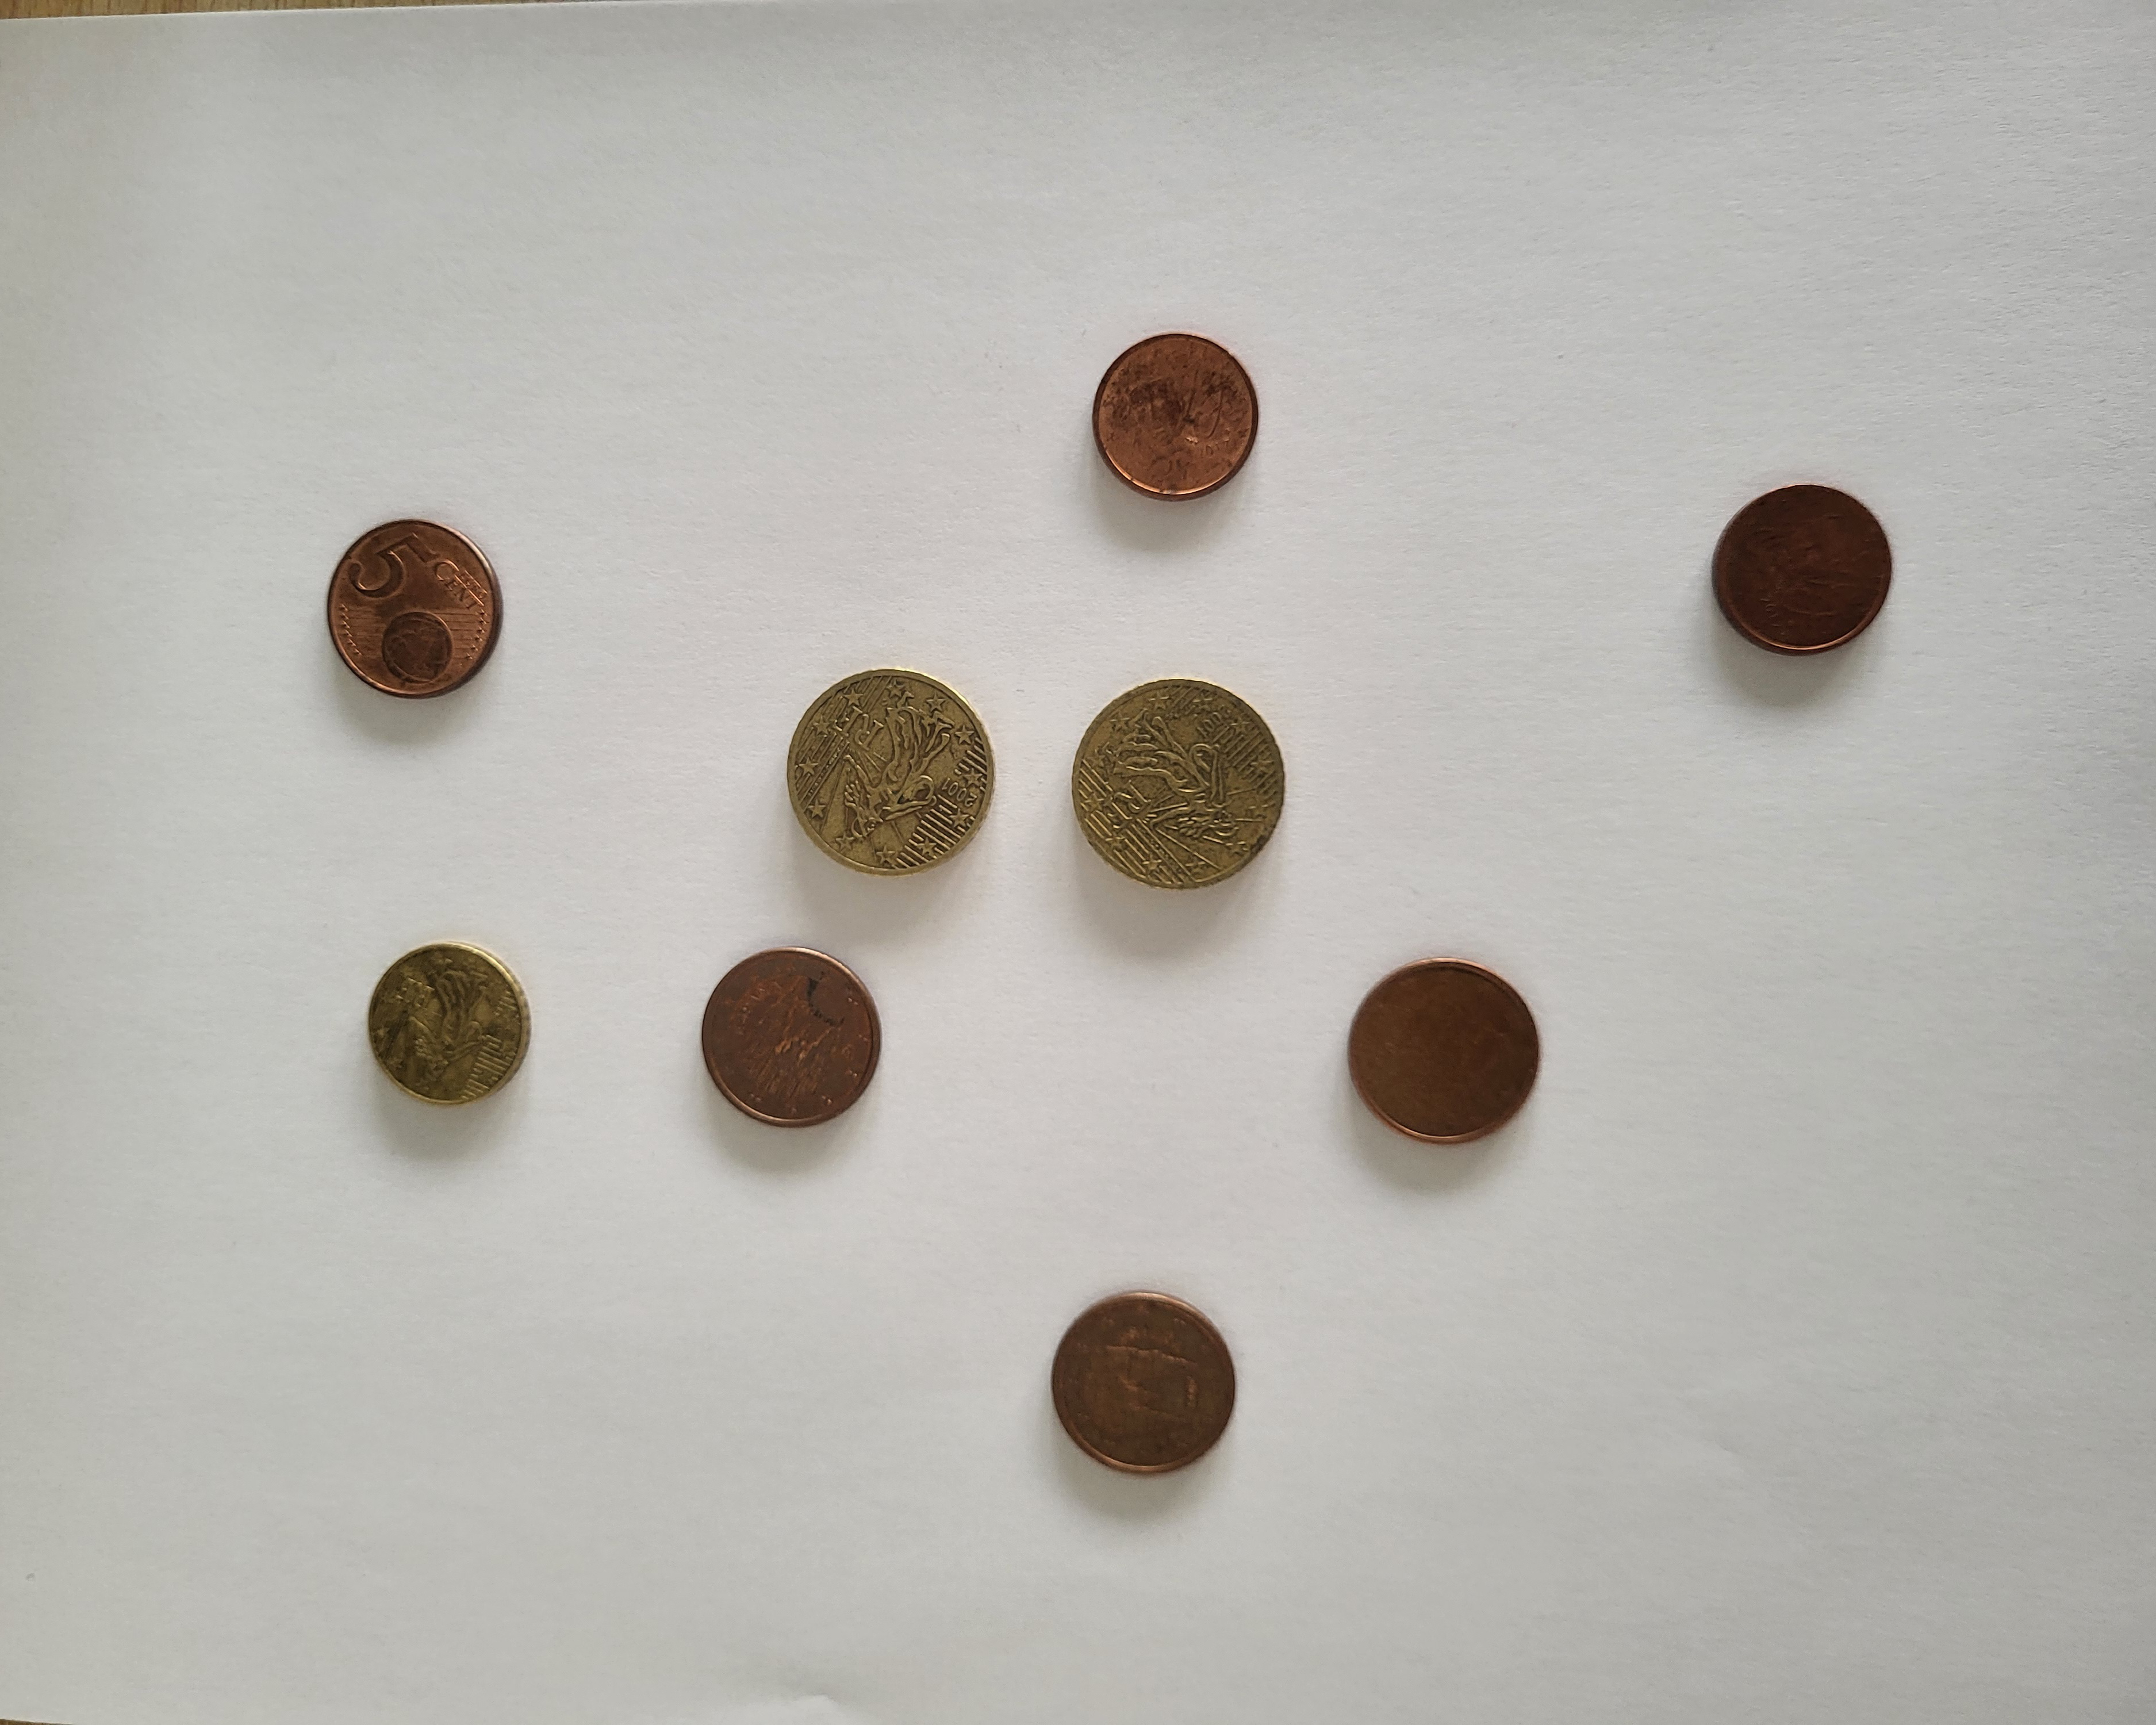
\includegraphics[width=0.8\textwidth]{./object/g1.png}
		\caption{Montage du réseau sur Filius}
	\end{figure}

	Ensuite on configure l'adresse IP de deux ordinateur, l'un sur \texttt{192.168.0.1} et l'autre sur \texttt{192.168.0.2}. En passant en mode simulation on ouvre le \texttt{PC2} et après avoir installé la ligne de commande on rentre les commandes suivantes : \texttt{ipconfig}, \texttt{arp -a} et \texttt{route}.
	\begin{items}{-15pt}{-10pt}
		\item \texttt{ipconfig} : Permet de regarder la configuration et les propriétés de la connexion de l'ordinateur sur le réseau
		\item \texttt{arp -a} : Permet de lister la table ARP de l'ordinateur
		\item \texttt{route} : Permet d'afficher la table de routage de l'ordinateur.
	\end{items}
	\begin{figure}[ht!]
	\minipage{0.32\textwidth}
	\adjustbox{width=0.95\textwidth}{
		\begin{tabular}{ l  l }
			Adresse IP  & : 192.168.0.2 \\
			Masque & : 255.255.255.0 \\
			Adresse MAC & : 24:CC:B6:3B:D6:C1 \\
			Passerelle & : 192.168.0.254 \\
			Serveur DNS & : 194.214.191.100			
		\end{tabular}
	}
	\endminipage\hfill
	\minipage{0.32\textwidth}
	\adjustbox{width=0.9\textwidth}{
		\begin{tabular}{ |c | c| }
			\hline
			Adresse IP  & Adresse Mac \\
			\hline
			255.255.255.255 & FF:FF:FF:FF:FF:FF \\
			\hline		
		\end{tabular}
	}
	\endminipage\hfill
	\minipage{0.32\textwidth}
	\adjustbox{width=0.95\textwidth}{
		\begin{tabular}{ |l | l| l| }
			\hline
			Destination & Masque & Passerelle\\
			\hline
			192.168.0.2 & 255.255.255.255 & 127.0.0.1 \\
			\hline		
			192.168.0.0 & 255.255.255.0 & 192.168.0.2\\
			\hline
			127.0.0.0 & 255.0.0.0 & 127.0.0.1\\
			\hline
			0.0.0.0 & 0.0.0.0 & 192.168.0.254\\
			\hline
		\end{tabular}
	}
	\endminipage\hfill
	\caption{Configuration IP, Table ARP et Table Routage}	
	\end{figure}
	
	Pour l'instant on voit que l'ordinateur est configuré avec l'IP correspondante. Sa table ARP ne contient que l'adresse IP et MAC du broadcast, autrement dit elle ne contient pas les adresses MAC d'autres ordinateurs sur le réseau. Finalement sa Table de routage nous indique que pour des trames dirigées à sa propre adresse utiliseras la passerelle locale, celles dirigées à un appareil sur le réseau seront envoyé à partir de la carte réseau et tout le reste sera redirigé ver l'adresse \texttt{192.168.0.254}.

	On effectue un ping entre l'ordinateur 2 et l'ordinateur 1, les échanges figurant ci-dessous:

	\begin{figure}[ht!]
		\begin{tabular}{|l|l|l|l|l|l|l|}
			\hline
			No. & Date & Source & Destination & Protocole & Couche & Commentaire\\
			\hline
			1 & 21:26:38:286 & 192.168.0.2 & 192.168.0.1 & ARP & Internet & Recherche MAC associée à 192.168.0.1\\
			\hline
			2 & 21:26:39:005 & 192.168.0.2 & 192.168.0.1 & ARP & Internet & Recherche MAC associée à 192.168.0.1\\
			\hline
			3 & 21:26:39:007 & 192.168.0.2 & 192.168.0.1 & ARP & Internet & Recherche MAC associée à 192.168.0.1\\
			\hline
			
		\end{tabular}
		\caption{Échange de Trames sans requête ARP}
	\end{figure}

	\begin{figure}[ht!]
		\begin{tabular}{|l|l|l|l|l|l|l|}
			\hline
			No. & Date & Source & Destination & Protocole & Couche & Commentaire\\
			\hline
			1 & 21:26:39:007 & 192.168.0.2 & 192.168.0.1 & ICMP & Internet & Echo Request (ping), TTL: 64, Seq.-No.: 1\\
			\hline
			2 & 21:26:39:532 & 192.168.0.1 & 192.168.0.2 & ICMP & Internet & Echo Reply (pong), TTL: 64, Seq.-No.: 1\\
			\hline
			  & & & \vdots & & & \\
			\hline
			8 & 21:26:42:049 & 192.168.0.1 & 192.168.0.2 & ICMP & Internet & Echo Reply (pong), TTL: 64, Seq.-No.: 4\\
			\hline
			
		\end{tabular}
		\caption{Échange de Trames sans requête ARP}
	\end{figure}
	\newpage
	On voit donc qu'une fois le premier ping et effectué entre les deux machine, l'ordinateur n'émet pas de requête ARP. Si nous regardons sa table ARP on retrouve :
	\begin{figure}[ht!]
		\centering
		\begin{tabular}{|c|c|}
			\hline
			Adresse IP & Adresse MAC\\
			\hline
			192.168.0.1 & F5:46:A5:C9:61:1C\\
			\hline
			255.255.255.255 & FF:FF:FF:FF:FF:FF\\
			\hline
		\end{tabular}
		\caption{Table ARP de l'ordinateur 2}
	\end{figure}
	
	On voit que l'adresse MAC de l'ordinateur 1 a été enregistrée dans la table ARP de l'ordinateur. Ceci explique pourquoi il n'a donc pas besoin de refaire une requête ARP; il connait déjà l'adresse MAC qui correspond à l'ordinateur 1.

	Q5. 

	\section{Mise en place du DHCP}

	On configure le \texttt{PC1} en tant que serveur DHCP avec une plage de \texttt{192.168.0.100} à \texttt{192.168.0.150}. Et on met le \texttt{PC3} en mode adressage automatique par serveur DHCP. Après la simulation on obtient observe les trames échangés:

	\begin{figure}[ht!]
		\centering
		\adjustbox{width=0.95\textwidth}{
		\begin{tabular}{|l|l|l|l|l|l|l|}
			\hline
			No. & Date & Source & Destination & Protocole & Couche & Commentaire\\
			\hline
			1 & 23:22:18.367 & 0.0.0.0:68 & 255.255.255.255:67 & DHCP & Application & DHCPDISCOVER yiaddr=0.0.0.0 chaddr=DB:43:7A:8E:3C:05\\
			\hline
			2 & 23:22:18:710 & 192.168.0.1:67 & 255.255.255.255:68 & DHCP & Application & DHCPOFFER yiaddr=192.168.0.100 chaddr=DB:43:7A:8E:3C:05\\
			\hline
			3 & 23:22:18.711 & 0.0.0.0 & 192.168.0.100 & ARP & Internet & Recherche MAC associée à 192.168.0.100\\
			\hline
			4 & 23:22:19.962 & 0.0.0.0 & 192.168.0.100 & ARP & Internet & Recherche MAC associée à 192.168.0.100\\
			\hline
			5 & 23:22:21.212 & 0.0.0.0:68 & 255.255.255.255:67 & DHCP & Application & DHCPREQUEST yiaddr=0.0.0.0 chaddr=DB:43:7A:8E:3C:05\\
			\hline
			6 & 23:22:21.520 & 192.168.0.1:67 & 255.255.255.255:68 & DHCP & Application & DHCPACK yiaddr=192.168.0.100 chaddr=DB:43:7A:8E:3C:05\\
			\hline
		\end{tabular}
	}
	\end{figure}

	Quand le \texttt{PC3} se connecte au réseau, envoi à l'IP de broadcast une découverte de serveur DHCP. Quand cette trame parvient au serveur il retourne aussi en broadcast une offre d'adresse IP et de passerelle. Le \texttt{PC3}vérifie ensuite que cette adresse ne soit pas occupée pas quelqu'un en envoyant une requête ARP à l'adresse IP qui lui est offerte. Quand il n'y a pas de réponse alors elle envoi une demande au serveur DHCP pour s'assigner l'adresse IP qui lui est offerte. Et après confirmation du serveur DHCP il modifie alors les configurations de sa connexion sur le réseau. 

	D'après ce tableau on peut donc bien voir que l'adresse qui lui est automatiquement affectée est la première dans la plage d'adresse : \texttt{192.168.0.100}. 

	\newpage

	\section{Configuration du Routeur}

	\begin{figure}[ht!]
		\centering
		\begin{tabular}{|c|c|c|c|}
			\hline
			IP de Destination & Masque & Passerelle & Interface\\
			\hline
			194.214.131.254 & 255.255.255.255 & 127.0.0.1 & 127.0.0.1\\
			\hline
			192.168.0.254 & 255.255.255.255 & 127.0.0.1 & 127.0.0.1\\
			\hline
			194.214.131.0 & 255.255.255.0 & 194.214.131.254 & 194.214.131.254\\
			\hline
			192.168.0.0 & 255.255.255.0 & 192.168.0.254 & 192.168.0.254\\
			\hline
			127.0.0.0 & 255.0.0.0 & 127.0.0.1 & 127.0.0.1\\
			\hline
		\end{tabular}
		\caption{Table de routage du routeur}
	\end{figure}

	Si un trame est à destination du router, c'est à dire avec l'IP \texttt{192.214.131.254} ou \texttt{192.168.0.254} alors le routeur utilise son interface et passerelle locale, il lit les trames qui lui sont destinés. Si une trame s'adresse à un appareil sur un deux deux réseaux alors il route cette trame vers le réseau correspondant en utilisant l'interface adequate. Et dernièrement s'il se parle a lui même il utilise sa passerelle et interface locale.
	
	On envoi maintenant un ping depuis le \texttt{PC2} au portable. On relève les trames suivantes:

	\begin{figure}[!ht]
		\centering
		\adjustbox{width=\textwidth}{
		\begin{tabular}{|l|l|l|l|l|l|l|l|}
			\hline
			No. & MAC Destination & MAC Source & IP Source & IP Destination & Protocole & Couche & Commentaire\\
			\hline
			1 & FF:FF:FF:FF:FF:FF & C2:FD:5A:E8:60:E5 & 192.168.0.2 & 192.168.0.254 & ARP & Internet & Requête ARP\\
			\hline
			2 & C2:FD:5A:E8:60:E5 & EF:36:DE:39:06:86 & 192.168.0.254 & 192.168.0.2 & ARP & Internet & Réponse ARP\\
			\hline
			3 & E8:36:DE:39:06:86 & C2:FD:5A:E8:60:E5 & 192.168.0.2 & 194.214.131.1 & ICMP & Internet & Echo Request\\
			\hline
			4 & C2:FD:5A:E8:60:E5 & EF:36:DE:39:06:86 & 194.214.131.1 & 192.168.0.2 & ICMP & Internet & Echo Reply\\
			\hline
			  & & & \vdots & & & \\
			  \hline
			10 & C2:FD:5A:E8:60:E5 & EF:36:DE:39:06:86 & 194.214.131.1 & 192.168.0.2 & ICMP & Internet & Echo Reply\\
			\hline
		\end{tabular}
	}
		\caption{Échanges de trames entre \texttt{PC2} et routeur}
	\end{figure}
	
	\begin{figure}[!ht]
		\centering
		\adjustbox{width=\textwidth}{
		\begin{tabular}{|l|l|l|l|l|l|l|l|}
			\hline
			No. & MAC Destination & MAC Source & IP Source & IP Destination & Protocole & Couche & Commentaire\\
			\hline
			1 & FF:FF:FF:FF:FF:FF & C1:47:C8:46:37:06 & 194.214.131.254 & 194.214.131.1 & ARP & Internet & Requête ARP\\
			\hline
			2 & C1:47:C8:46:37:06 & 8B:61:E6:30:57:33 & 194.214.131.1 & 194.214.131.254 & ARP & Internet & Réponse ARP\\
			\hline
			3 & E8:36:DE:39:06:86 & C1:47:C8:46:37:06 & 192.168.0.2 & 194.214.131.1 & ICMP & Internet & Echo Request\\
			\hline
			4 & C1:47:C8:46:37:06 & 8B:61:E6:30:57:33 & 194.214.131.1 & 192.168.0.2 & ICMP & Internet & Echo Reply\\
			\hline
			  & & & \vdots & & & \\
			  \hline
			10 & C1:47:C8:46:37:06 & 8B:61:E6:30:57:33 & 194.214.131.1 & 192.168.0.2 & ICMP & Internet & Echo Reply\\
			\hline
		\end{tabular}
	}
		\caption{Échanges de trames entre portable et routeur}
	\end{figure}

	Entre le \texttt{PC2} et le routeur on voit qu'il y a d'abord un requête ARP pour obtenir l'adresse MAC du routeur. Après l'avoir reçue il envoi un ping au portable mais avec une adresse MAC de destination du routeur. Lorsque le ping revient, c'est toujours l'adresse MAC du routeur qui est l'adresse source. 

	Quand on regarde avec les échanges entre le routeur et le portable on observe que la même chose se passe. Après une requête et une réponse ARP, le ping est envoyé avec l'adresse MAC du routeur et la destination de pong l'est aussi. 

	Le routeur agit donc comme un pont en se faisant passer par la machine mais en utilisant sa propre adresse MAC. 

	\section{Mise en oeuvre d'un DNS}

	Un serveur DNS permet d'associer un URL à une adresse IP, c'est à base de traduction.

	L'option "activer la résolution recursive de domaine" permet d'accéder à d'autre sites web en contactant d'autre serveur DNS, de cette façon on ne doit pas se reposer sur un unique serveur DNS. 
	
	\begin{figure}[ht!]
		\centering
		\includegraphics[width=0.7\textwidth]{./object/t2.png}
		\caption{Trames échangés}
	\end{figure}

	On constate qu'avant d'accéder au domaine il y a une demande au serveur DNS pour obtenir l'adresse IP du site, et ensuite le serveur répond avec l'IP du site. 

	Le protocole RIP consiste à ce que chaque routeur envoi sa table de routage au prochain, ceci permet d'optimiser le routage dans des réseaux complexes avec plusieurs routeur.

	Q18. La trame est un broadcast dans lequel est contenu l'IP du routeur et l'IP des autres machine auquel il est connecté 

	Si R11 est coupé alors les trames devrons prendre un chemin plus long pour arriver à leur déstinataires. 


\end{document}
